
Let \(V\) be the Euclidean space containing the root system \(\Delta\), and let
\(\alpha\in \Delta\). Since
\[
    (\alpha,\alpha)\neq 0,
\]
we have
\[
    V=\ker(\alpha)\oplus F\alpha,
\]
where
\[
    \ker(\alpha):=\{x\in V\mid (x,\alpha)=0\}.
\]

We define the reflection \(s_\alpha:V\to V\) by
\[
    s_\alpha(x)=x-\frac{2(x,\alpha)}{(\alpha,\alpha)}\alpha.
\]
From the previous discussion, we already know that
\[
    s_\alpha(\Delta)=\Delta.
\]

\begin{figure}[h]
    \centering
    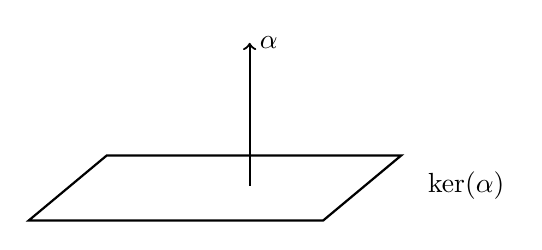
\begin{tikzpicture}[scale=1.1]
        % hyperplane
        \draw[thick] (-2.2,-0.6) -- (1.2,-0.6) -- (2.1,0.15) -- (-1.3,0.15) -- cycle;
        % normal vector
        \draw[thick,->] (0.35,-0.2) -- (0.35,1.45) node[right] {\(\alpha\)};
        % labels
        \node at (2.85,-0.2) {\(\ker(\alpha)\)};
    \end{tikzpicture}
    \caption{The hyperplane \(\ker(\alpha)\) and the normal vector \(\alpha\).}
\end{figure}

\begin{lemma}
    One has
    \[
        \operatorname{span}(\Delta)=H^*.
    \]
\end{lemma}

\begin{proof}
    Suppose \(\operatorname{span}(\Delta)\neq H^*\). Then there exists
    \[
        0\neq h\in H
    \]
    such that
    \[
        \gamma(h)=0
        \qquad
        \text{for all }\gamma\in \operatorname{span}(\Delta).
    \]
    In particular,
    \[
        \alpha(h)=0
        \qquad
        \text{for all }\alpha\in \Delta.
    \]
    Hence \(h\) commutes with all root vectors \(x_\alpha\). Since \(h\in H\), it also
    commutes with \(H\). Therefore \(h\) commutes with all of \(L\), so
    \[
        h\in Z(L).
    \]
    But \(L\) is semisimple, hence \(Z(L)=0\). This is a contradiction. Therefore
    \[
        \operatorname{span}(\Delta)=H^*.
    \]
\end{proof}

\begin{lemma}
    For all \(\alpha,\beta\in \Delta\), one has
    \[
        (\alpha,\beta)\in \mathbb{Q}.
    \]
\end{lemma}

\begin{proof}
    Recall that
    \[
        \frac{2(\alpha,\beta)}{(\alpha,\alpha)}\in \mathbb{Z}.
    \]
    Thus it suffices to prove that
    \[
        (\alpha,\alpha)\in \mathbb{Q}
        \qquad
        \text{for all }\alpha\in \Delta.
    \]

    Let \(\nu:H\to H^*\) be the isomorphism induced by the Killing form \(B\), and
    write
    \[
        t_\alpha:=\nu^{-1}(\alpha)\in H.
    \]
    Then
    \[
        h_\alpha=\frac{2}{(\alpha,\alpha)}\,t_\alpha.
    \]
    Now
    \[
        (\alpha,\alpha)
        =
        B(t_\alpha,t_\alpha)
        =
        \operatorname{Tr}\!\bigl((\operatorname{ad}t_\alpha)^2\bigr)
        =
        \sum_{\beta\in\Delta}\beta(t_\alpha)^2.
    \]
    Since
    \[
        \beta(t_\alpha)=\frac{(\alpha,\alpha)}{2}\,\beta(h_\alpha),
    \]
    we obtain
    \[
        (\alpha,\alpha)
        =
        \frac{(\alpha,\alpha)^2}{4}
        \sum_{\beta\in\Delta}\beta(h_\alpha)^2.
    \]
    Therefore
    \[
        \frac{4}{(\alpha,\alpha)}
        =
        \sum_{\beta\in\Delta}\beta(h_\alpha)^2
        \in \mathbb{Q},
    \]
    because each \(\beta(h_\alpha)\in \mathbb{Z}\). Hence
    \[
        (\alpha,\alpha)\in \mathbb{Q}.
    \]
    It now follows that
    \[
        (\alpha,\beta)
        =
        \frac{(\alpha,\alpha)}{2}\,\beta(h_\alpha)\in \mathbb{Q}.
    \]
\end{proof}

Now consider
\[
    E:=\sum_{\alpha\in\Delta}\mathbb{Q}\alpha \subseteq H^*.
\]
Choose \(\alpha_1,\dots,\alpha_n\in \Delta\) such that
\[
    \{\alpha_1,\dots,\alpha_n\}
\]
is an \(F\)-basis of \(H^*\). For any \(\beta\in \Delta\), write
\[
    \beta=\sum_{i=1}^n k_i\alpha_i,
    \qquad
    k_i\in F.
\]

\begin{lemma}
    Each coefficient \(k_i\) lies in \(\mathbb{Q}\).
\end{lemma}

\begin{proof}
    For \(j=1,\dots,n\), we have
    \[
        (\beta,\alpha_j)=\sum_{i=1}^n k_i(\alpha_i,\alpha_j).
    \]
    This is a system of \(n\) linear equations in the unknowns \(k_1,\dots,k_n\),
    whose coefficients lie in \(\mathbb{Q}\), since by the previous lemma
    \[
        (\beta,\alpha_j)\in\mathbb{Q},
        \qquad
        (\alpha_i,\alpha_j)\in\mathbb{Q}.
    \]
    Because the form \((\cdot,\cdot)\) is nondegenerate, the Gram matrix
    \[
        \bigl((\alpha_i,\alpha_j)\bigr)_{1\le i,j\le n}
    \]
    is invertible. Hence the system has a unique solution, and this solution lies in
    \(\mathbb{Q}\). Therefore
    \[
        k_i\in \mathbb{Q}
        \qquad
        \text{for all }i.
    \]
\end{proof}

\begin{corollary}
    One has
    \[
        \dim_{\mathbb{Q}}\!\left(\sum_{\alpha\in\Delta}\mathbb{Q}\alpha\right)
        =
        \dim_F H^*.
    \]
\end{corollary}

\begin{proof}
    Let
    \[
        n=\dim_F H^*.
    \]
    Since
    \[
        \operatorname{span}_F(\Delta)=H^*,
    \]
    we may choose roots
    \[
        \alpha_1,\dots,\alpha_n\in\Delta
    \]
    which form an \(F\)-basis of \(H^*\).

    First, \(\alpha_1,\dots,\alpha_n\) are \(\mathbb{Q}\)-linearly independent.
    Indeed, if
    \[
        q_1\alpha_1+\cdots+q_n\alpha_n=0,
        \qquad q_i\in\mathbb{Q},
    \]
    then this is also an \(F\)-linear relation. Since
    \(\alpha_1,\dots,\alpha_n\) are \(F\)-linearly independent, we get
    \[
        q_1=\cdots=q_n=0.
    \]
    Hence
    \[
        \dim_{\mathbb{Q}}\!\left(\sum_{\alpha\in\Delta}\mathbb{Q}\alpha\right)
        \geq n.
    \]

    Conversely, by the preceding lemma, every \(\beta\in\Delta\) can be written as
    \[
        \beta=\sum_{i=1}^n k_i\alpha_i
    \]
    with
    \[
        k_i\in\mathbb{Q}.
    \]
    Therefore
    \[
        \sum_{\alpha\in\Delta}\mathbb{Q}\alpha
        =
        \sum_{i=1}^n \mathbb{Q}\alpha_i.
    \]
    Thus
    \[
        \dim_{\mathbb{Q}}\!\left(\sum_{\alpha\in\Delta}\mathbb{Q}\alpha\right)
        \leq n.
    \]
    Combining the two inequalities gives
    \[
        \dim_{\mathbb{Q}}\!\left(\sum_{\alpha\in\Delta}\mathbb{Q}\alpha\right)
        =
        n
        =
        \dim_F H^*.
    \]
\end{proof}

\begin{lemma}
    The restriction of \((\cdot,\cdot)\) to
    \[
        \sum_{\alpha\in\Delta}\mathbb{Q}\alpha
    \]
    is positive definite.
\end{lemma}

\begin{proof}
    Let
    \[
        0\neq \lambda\in \sum_{\alpha\in\Delta}\mathbb{Q}\alpha,
    \]
    and let \(t_\lambda:=\nu^{-1}(\lambda)\in H\). Then
    \[
        (\lambda,\lambda)
        =
        B(t_\lambda,t_\lambda)
        =
        \operatorname{Tr}\!\bigl((\operatorname{ad}t_\lambda)^2\bigr)
        =
        \sum_{\alpha\in\Delta}\alpha(t_\lambda)^2
        \ge 0.
    \]
    If \((\lambda,\lambda)=0\), then
    \[
        \alpha(t_\lambda)=0
        \qquad
        \text{for all }\alpha\in\Delta.
    \]
    By the lemma \(\operatorname{span}(\Delta)=H^*\), this implies \(t_\lambda=0\),
    hence \(\lambda=0\), a contradiction. Therefore
    \[
        (\lambda,\lambda)>0
        \qquad
        \text{for all }0\neq \lambda\in \sum_{\alpha\in\Delta}\mathbb{Q}\alpha.
    \]
    Thus the form is positive definite on
    \[
        \sum_{\alpha\in\Delta}\mathbb{Q}\alpha.
    \]
\end{proof}

Let
\[
    E_{\mathbb{Q}}
    :=
    \sum_{\alpha\in\Delta}\mathbb{Q}\alpha
    \subseteq H^*.
\]
By the preceding corollary,
\[
    \dim_{\mathbb{Q}}E_{\mathbb{Q}}
    =
    \dim_F H^*.
\]
We now extend \(E_{\mathbb{Q}}\) to a real vector space by setting
\[
    E
    :=
    E_{\mathbb{Q}}\otimes_{\mathbb{Q}}\mathbb{R}.
\]
Thus \(E\) is a finite-dimensional real vector space.

The symmetric bilinear form \((\cdot,\cdot)\) on \(E_{\mathbb{Q}}\) extends
naturally to an \(\mathbb{R}\)-bilinear form on \(E\) by
\[
    \left(
    \sum_i v_i\otimes r_i,\,
    \sum_j w_j\otimes r'_j
    \right)
    :=
    \sum_{i,j} (v_i,w_j) r_i r'_j,
\]
where
\[
    v_i,w_j\in E_{\mathbb{Q}},
    \qquad
    r_i,r'_j\in \mathbb{R}.
\]

This form is positive definite. Indeed, if
\[
    \alpha_1,\dots,\alpha_n
\]
is a \(\mathbb{Q}\)-basis of \(E_{\mathbb{Q}}\), then it is also an
\(\mathbb{R}\)-basis of \(E\). With respect to this basis, the Gram matrix of
the extended form is still
\[
    \bigl((\alpha_i,\alpha_j)\bigr)_{1\le i,j\le n}.
\]
Since the original form is positive definite on \(E_{\mathbb{Q}}\), this
matrix is positive definite. Hence the extended form is positive definite on
\(E\). Therefore \(E\) is a Euclidean space.

\subsection{Abstract Root Systems}

\begin{definition}[Root system]
    Let \(E=\mathbb{R}^n\) be a Euclidean space with inner product
    \((\cdot,\cdot)\). A subset \(\Delta\subseteq E\) is called a \emph{root system}
    if the following conditions hold:
    \begin{enumerate}
        \item
              \[
                  \Delta\subseteq E\setminus\{0\},
                  \qquad
                  |\Delta|<\infty.
              \]

        \item
              \[
                  \operatorname{span}_{\mathbb{R}}(\Delta)=E.
              \]

        \item
              For every \(\alpha\in\Delta\),
              \[
                  s_\alpha(\Delta)=\Delta,
              \]
              where
              \[
                  s_\alpha(x)
                  =
                  x-\frac{2(x,\alpha)}{(\alpha,\alpha)}\alpha
              \]
              is the reflection with respect to the hyperplane orthogonal to \(\alpha\).

        \item
              For all \(\alpha,\beta\in\Delta\),
              \[
                  \frac{2(\alpha,\beta)}{(\alpha,\alpha)}\in\mathbb{Z}.
              \]

        \item
              For every \(\alpha\in\Delta\),
              \[
                  \mathbb{R}\alpha\cap\Delta
                  =
                  \{\alpha,-\alpha\}.
              \]
    \end{enumerate}
\end{definition}

For the moment, we forget the Lie algebra and work only with abstract root
systems.

\begin{definition}[Irreducible root system]
    Let \(\Delta\subseteq E\) be a root system in a Euclidean space \(E\). We say
    that \(\Delta\) is \emph{irreducible} if it cannot be written as a disjoint union
    \[
        \Delta=\Delta_1\cup\Delta_2,
    \]
    where \(\Delta_1,\Delta_2\) are nonempty subsets satisfying
    \[
        (\Delta_1,\Delta_2)=0.
    \]
    Equivalently, \(\Delta\) is irreducible if \(E\) cannot be decomposed as an
    orthogonal direct sum
    \[
        E=\operatorname{span}_{\mathbb{R}}(\Delta_1)
        \oplus
        \operatorname{span}_{\mathbb{R}}(\Delta_2)
    \]
    with roots split between the two summands.
\end{definition}

\begin{example}
    In dimension \(1\), there is only one root system:
    \[
        \Delta=\{\alpha,-\alpha\}.
    \]
    \[
        \begin{tikzpicture}[scale=1.1, >=Stealth]
            \draw[->] (-2,0) -- (2,0);
            \draw[->, thick] (0,0) -- (1.2,0) node[above] {\(\alpha\)};
            \draw[->, thick] (0,0) -- (-1.2,0) node[above] {\(-\alpha\)};
            \fill (0,0) circle (1.2pt);
        \end{tikzpicture}
    \]
\end{example}

\begin{example}
    Typical irreducible root systems in dimension \(2\) include the following
    pictures.

    \[
        \begin{tikzpicture}[scale=1.15, >=Stealth]
            % B2-type diagram
            \foreach \x/\y in {1/0,-1/0,0/1,0/-1,1/1,-1/1,1/-1,-1/-1}
                {
                    \draw[->, thick] (0,0) -- (\x,\y);
                }
            \draw (-1,-1) -- (1,-1) -- (1,1) -- (-1,1) -- cycle;
            \draw[gray!60] (-1,0) -- (1,0);
            \draw[gray!60] (0,-1) -- (0,1);
            \fill (0,0) circle (1pt);
        \end{tikzpicture}
        \qquad
        \begin{tikzpicture}[scale=1.0, >=Stealth]
            % G2-type diagram
            \foreach \a in {0,60,...,300}
                {
                    \draw[->, thick] (0,0) -- ({1.45*cos(\a)},{1.45*sin(\a)});
                }
            \foreach \a in {30,90,...,330}
                {
                    \draw[->, thick] (0,0) -- ({0.9*cos(\a)},{0.9*sin(\a)});
                }
            \foreach \a in {0,60,...,300}
                {
                    \draw[gray!60] ({1.45*cos(\a)},{1.45*sin(\a)}) --
                    ({1.45*cos(\a+60)},{1.45*sin(\a+60)});
                }
            \fill (0,0) circle (1pt);
        \end{tikzpicture}
    \]
\end{example}

We now study possible angles between two roots. Let
\[
    \alpha,\beta\in\Delta
\]
satisfy
\[
    (\alpha,\beta)\neq 0,
    \qquad
    \beta\neq \pm \alpha.
\]
Let \(\theta\) be the angle between \(\alpha\) and \(\beta\). Then
\[
    (\alpha,\beta)
    =
    \|\alpha\|\,\|\beta\|\cos\theta.
\]

By the axioms of a root system,
\[
    \frac{2(\beta,\alpha)}{(\alpha,\alpha)}\in\mathbb{Z},
    \qquad
    \frac{2(\alpha,\beta)}{(\beta,\beta)}\in\mathbb{Z}.
\]
Multiplying these two integers gives
\[
    \frac{2(\beta,\alpha)}{(\alpha,\alpha)}
    \cdot
    \frac{2(\alpha,\beta)}{(\beta,\beta)}
    =
    \frac{4(\alpha,\beta)^2}{(\alpha,\alpha)(\beta,\beta)}
    =
    4\cos^2\theta.
\]
Since \(\beta\neq \pm\alpha\), this product cannot be \(4\). Since
\((\alpha,\beta)\neq 0\), it is nonzero. Hence
\[
    4\cos^2\theta\in\{1,2,3\}.
\]
Therefore
\[
    \cos^2\theta\in
    \left\{
    \frac14,\frac12,\frac34
    \right\}.
\]
Thus the possible non-right, nonzero angles are
\[
    \theta
    \in
    \left\{
    \frac{\pi}{6},
    \frac{\pi}{4},
    \frac{\pi}{3},
    \frac{2\pi}{3},
    \frac{3\pi}{4},
    \frac{5\pi}{6}
    \right\}.
\]

In particular, at least one of the two integers
\[
    \frac{2(\beta,\alpha)}{(\alpha,\alpha)},
    \qquad
    \frac{2(\alpha,\beta)}{(\beta,\beta)}
\]
has absolute value \(1\). Replacing \(\beta\) by \(-\beta\) if necessary, we may
assume
\[
    (\alpha,\beta)>0.
\]
Without loss of generality, suppose
\[
    \frac{2(\beta,\alpha)}{(\alpha,\alpha)}=1.
\]
Then
\[
    1
    =
    \frac{2\|\beta\|\|\alpha\|\cos\theta}{\|\alpha\|^2}
    =
    \frac{2\|\beta\|\cos\theta}{\|\alpha\|}.
\]
Hence
\[
    \frac{\|\alpha\|}{\|\beta\|}
    =
    2\cos\theta.
\]
Consequently,
\[
    \cos\theta=\frac12
    \quad\Longrightarrow\quad
    \|\alpha\|=\|\beta\|,
\]
\[
    \cos\theta=\frac{\sqrt2}{2}
    \quad\Longrightarrow\quad
    \|\alpha\|=\sqrt2\,\|\beta\|,
\]
and
\[
    \cos\theta=\frac{\sqrt3}{2}
    \quad\Longrightarrow\quad
    \|\alpha\|=\sqrt3\,\|\beta\|.
\]
Thus the possible ratios of root lengths are
\[
    1,\qquad \sqrt2,\qquad \sqrt3.
\]

Let \(E=\mathbb{R}^n\) be a Euclidean space with inner product
\((\cdot,\cdot)\), and let \(\Delta\subset E\) be a root system.

\begin{definition}[Base]
    A subset
    \[
        B=\{\beta_1,\ldots,\beta_n\}\subset \Delta
    \]
    is called a \emph{base} of \(\Delta\) if the following two conditions hold:
    \begin{enumerate}
        \item \(B\) is a basis of \(E\);
        \item for every \(\alpha\in\Delta\), one has
              \[
                  \alpha=k_1\beta_1+\cdots+k_n\beta_n
              \]
              where either all \(k_i\in\mathbb{Z}_{\geq 0}\), or all
              \(k_i\in\mathbb{Z}_{\leq 0}\).
    \end{enumerate}
    In this case one obtains a decomposition
    \[
        \Delta=\Delta^+\dot\cup \Delta^-,
    \]
    where
    \[
        \Delta^+
        =
        \Delta\cap
        \sum_{i=1}^n \mathbb{Z}_{\geq 0}\beta_i,
        \qquad
        \Delta^-=-\Delta^+.
    \]
\end{definition}

\begin{lemma}
    Let \(B\) be a base of \(\Delta\). If \(\beta_1,\beta_2\in B\) and
    \(\beta_1\neq \beta_2\), then
    \[
        (\beta_1,\beta_2)\leq 0.
    \]
    Equivalently, the angle between two distinct elements of \(B\) is obtuse or
    right.
\end{lemma}

\begin{proof}
    Suppose, to the contrary, that
    \[
        (\beta_1,\beta_2)>0.
    \]
    Then the Cartan integer
    \[
        \frac{2(\beta_1,\beta_2)}{(\beta_2,\beta_2)}
    \]
    is a positive integer. Since \(\Delta\) is stable under reflections, we have
    \[
        s_{\beta_2}(\beta_1)
        =
        \beta_1
        -
        \frac{2(\beta_1,\beta_2)}{(\beta_2,\beta_2)}\beta_2
        \in \Delta.
    \]
    But relative to the basis \(B\), this root has coefficient \(1>0\) on
    \(\beta_1\) and a negative coefficient on \(\beta_2\). This contradicts the
    definition of a base, since every root must be either a nonnegative or a
    nonpositive integral linear combination of the elements of \(B\). Therefore
    \[
        (\beta_1,\beta_2)\leq 0.
    \]
\end{proof}

\begin{example}
    The following diagrams illustrate possible choices of bases in rank \(2\).

    \[
        \begin{tikzpicture}[scale=0.85,>=Stealth]
            \coordinate (O) at (0,0);

            % B2 roots
            \draw[->, very thick] (O) -- (1.4,0)
            node[right] {\(\alpha\)};
            \draw[->, very thick] (O) -- (-1.4,1.4)
            node[above left] {\(\beta\)};

            \draw[->] (O) -- (0,1.4)
            node[above] {\(\alpha+\beta\)};
            \draw[->] (O) -- (1.4,1.4)
            node[above right] {\(2\alpha+\beta\)};

            \draw[->] (O) -- (-1.4,0)
            node[left] {\(-\alpha\)};
            \draw[->] (O) -- (1.4,-1.4)
            node[below right] {\(-\beta\)};
            \draw[->] (O) -- (0,-1.4)
            node[below] {\(-\alpha-\beta\)};
            \draw[->] (O) -- (-1.4,-1.4)
            node[below left] {\(-2\alpha-\beta\)};

            \fill (O) circle (1.2pt);
            \node at (0,-2.2) {\(B_2\)};
        \end{tikzpicture}
        \qquad\qquad
        \begin{tikzpicture}[scale=0.75,>=Stealth]
            \coordinate (O) at (0,0);

            % positive roots of G2
            \draw[->, very thick] (O) -- (1.2,0)
            node[right] {\(\alpha\)};
            \draw[->, very thick] (O) -- (-1.8,1.04)
            node[above left] {\(\beta\)};

            \draw[->] (O) -- (-0.6,1.04)
            node[above left] {\(\alpha+\beta\)};
            \draw[->] (O) -- (0.6,1.04)
            node[above right] {\(2\alpha+\beta\)};
            \draw[->] (O) -- (1.8,1.04)
            node[above right] {\(3\alpha+\beta\)};
            \draw[->] (O) -- (0,2.08)
            node[above] {\(3\alpha+2\beta\)};

            % negative roots
            \draw[->] (O) -- (-1.2,0);
            \draw[->] (O) -- (1.8,-1.04);
            \draw[->] (O) -- (0.6,-1.04);
            \draw[->] (O) -- (-0.6,-1.04);
            \draw[->] (O) -- (-1.8,-1.04);
            \draw[->] (O) -- (0,-2.08);

            \fill (O) circle (1.2pt);
            \node at (0,-2.65) {\(G_2\)};
        \end{tikzpicture}
    \]
\end{example}

\begin{lemma}
    Let \(F\) be an infinite field and let \(V\) be a finite-dimensional vector
    space over \(F\). Then \(V\) is not the union of finitely many proper
    hyperplanes.
\end{lemma}

\begin{proof}
    Suppose, to the contrary, that
    \[
        V=V_1\cup\cdots\cup V_m
    \]
    where each \(V_i\) is a proper hyperplane. We may assume that no \(V_i\) is
    contained in the union of the others.

    Choose
    \[
        y\in V_1\setminus \bigcup_{i=2}^m V_i.
    \]
    Since \(V_1\neq V\), choose \(x\notin V_1\). Consider the affine line
    \[
        y+Fx=\{y+ax\mid a\in F\}.
    \]
    This line meets \(V_1\) only at \(y\), because if \(y+ax\in V_1\) and
    \(a\neq 0\), then \(x\in V_1\), a contradiction. Moreover, for each
    \(i\geq 2\), the line \(y+Fx\) meets \(V_i\) in at most one point, since
    \(y\notin V_i\).

    Thus the finite union \(V_1\cup\cdots\cup V_m\) meets the line \(y+Fx\) in
    only finitely many points. Since \(F\) is infinite, there exists \(a\in F\)
    such that
    \[
        y+ax\notin V_1\cup\cdots\cup V_m,
    \]
    a contradiction.
\end{proof}

\begin{lemma}
    Let \(\alpha,\beta\in\Delta\) with \(\alpha\neq\beta\). If
    \[
        \alpha-\beta\notin\Delta,
    \]
    then
    \[
        (\alpha,\beta)\leq 0.
    \]
\end{lemma}

\begin{proof}
    By the root-string property, the \(\beta\)-string through \(\alpha\) has the
    form
    \[
        \alpha-r\beta,\ldots,\alpha,\ldots,\alpha+q\beta,
    \]
    where \(r,q\in\mathbb{Z}_{\geq 0}\), and
    \[
        r-q
        =
        \frac{2(\alpha,\beta)}{(\beta,\beta)}.
    \]
    Since \(\alpha-\beta\notin\Delta\), one has \(r=0\). Hence
    \[
        \frac{2(\alpha,\beta)}{(\beta,\beta)}
        =
        -q
        \leq 0.
    \]
    Since \((\beta,\beta)>0\), it follows that
    \[
        (\alpha,\beta)\leq 0.
    \]
\end{proof}

\begin{lemma}
    Let \(S=\{s_1,\ldots,s_m\}\) be a finite set of nonzero vectors in a
    Euclidean space. Suppose that
    \[
        (s_i,s_j)\leq 0
        \qquad
        \text{for all } i\neq j,
    \]
    and suppose that there exists \(f\neq 0\) such that
    \[
        (f,s_i)>0
        \qquad
        \text{for all } i.
    \]
    Then \(S\) is linearly independent.
\end{lemma}

\begin{proof}
    Suppose that
    \[
        \sum_{i=1}^m k_i s_i=0
    \]
    for some \(k_i\in\mathbb{R}\), not all zero. If all nonzero \(k_i\) have the
    same sign, then pairing with \(f\) gives an immediate contradiction.

    Thus, after separating positive and negative coefficients, we may write
    \[
        \sum_{i\in I} k_i s_i
        =
        \sum_{j\in J} h_j s_j,
    \]
    where \(I\cap J=\varnothing\) and all \(k_i,h_j>0\). Set
    \[
        v=\sum_{i\in I} k_i s_i
        =
        \sum_{j\in J} h_j s_j.
    \]
    Then
    \[
        0\leq (v,v)
        =
        \left(
        \sum_{i\in I} k_i s_i,
        \sum_{j\in J} h_j s_j
        \right)
        =
        \sum_{i\in I,\ j\in J} k_i h_j (s_i,s_j)
        \leq 0.
    \]
    Hence \((v,v)=0\), so \(v=0\). But then
    \[
        0=(f,v)=\sum_{i\in I} k_i(f,s_i)>0,
    \]
    a contradiction. Therefore \(S\) is linearly independent.
\end{proof}

\begin{theorem}[Existence of a base]
    Every root system \(\Delta\subset E\) admits a base.
\end{theorem}

\begin{proof}
    First note that
    \[
        \bigcup_{\alpha\in\Delta}\alpha^\perp
        \neq E.
    \]
    Indeed, \(\Delta\) is finite, and each \(\alpha^\perp\) is a proper
    hyperplane. Hence the previous lemma applies.

    Choose
    \[
        \gamma\in E\setminus \bigcup_{\alpha\in\Delta}\alpha^\perp.
    \]
    Such a vector \(\gamma\) is called \emph{regular}. Thus
    \[
        (\gamma,\alpha)\neq 0
        \qquad
        \text{for all } \alpha\in\Delta.
    \]
    Define
    \[
        \Delta^+
        =
        \{\alpha\in\Delta\mid (\gamma,\alpha)>0\},
        \qquad
        \Delta^-
        =
        \{\alpha\in\Delta\mid (\gamma,\alpha)<0\}.
    \]
    Then
    \[
        \Delta=\Delta^+\dot\cup\Delta^-,
        \qquad
        \Delta^-=-\Delta^+.
    \]

    Now define
    \[
        B
        =
        \left\{
        \beta\in\Delta^+
        \ \middle|\
        \beta \text{ is not a sum of two elements of } \Delta^+
        \right\}.
    \]
    We claim that \(B\) is a base of \(\Delta\).

    First, \(B\neq\varnothing\). Indeed, since \(\Delta^+\) is finite, choose
    \(\beta\in\Delta^+\) such that
    \[
        (\gamma,\beta)
        =
        \min\{(\gamma,\alpha)\mid \alpha\in\Delta^+\}.
    \]
    If \(\beta=\alpha_1+\alpha_2\) with \(\alpha_1,\alpha_2\in\Delta^+\), then
    \[
        (\gamma,\alpha_i)>0
        \qquad
        (i=1,2),
    \]
    and hence
    \[
        (\gamma,\alpha_i)<(\gamma,\beta),
    \]
    contradicting the minimality of \(\beta\). Thus \(\beta\in B\).

    Next, every element of \(\Delta^+\) is a nonnegative integral linear
    combination of elements of \(B\). Indeed, if \(\alpha\in\Delta^+\) and
    \(\alpha\notin B\), then
    \[
        \alpha=\alpha_1+\alpha_2
    \]
    for some \(\alpha_1,\alpha_2\in\Delta^+\). Repeating this process, and using
    the finiteness of \(\Delta^+\), we eventually express \(\alpha\) as a sum of
    elements of \(B\). Since \(\Delta^-=-\Delta^+\), every negative root is a
    nonpositive integral linear combination of elements of \(B\).

    It remains to prove that \(B\) is linearly independent. Let
    \(\beta_1,\beta_2\in B\) with \(\beta_1\neq\beta_2\). We first show that
    \[
        \beta_1-\beta_2\notin\Delta.
    \]
    If \(\beta_1-\beta_2\in\Delta^+\), then
    \[
        \beta_1=\beta_2+(\beta_1-\beta_2),
    \]
    contradicting the definition of \(B\). If
    \(\beta_1-\beta_2\in\Delta^-\), then
    \[
        \beta_2=\beta_1+(\beta_2-\beta_1),
    \]
    again contradicting the definition of \(B\). Hence
    \[
        \beta_1-\beta_2\notin\Delta.
    \]
    By the previous lemma,
    \[
        (\beta_1,\beta_2)\leq 0.
    \]
    Moreover, since \(B\subset \Delta^+\), one has
    \[
        (\gamma,\beta)>0
        \qquad
        \text{for all } \beta\in B.
    \]
    Therefore, by the linear independence lemma, \(B\) is linearly independent.

    Finally, \(B\) spans \(\Delta\), and \(\Delta\) spans \(E\). Hence \(B\) is a
    basis of \(E\). We have already shown that every root is either a
    nonnegative or a nonpositive integral linear combination of elements of
    \(B\). Thus \(B\) is a base of \(\Delta\).
\end{proof}

